\documentclass[conference]{IEEEtran}

\usepackage[noadjust]{cite}
\usepackage{balance}

\IEEEoverridecommandlockouts
%
\usepackage{graphicx}
% If possible, figure files should be included in EPS format.
%
\usepackage{amsmath}
%
% If you use the hyperref package, please uncomment the following line
% to display URLs in blue roman font according to Springer's eBook style:
\usepackage{hyperref,xcolor}
\renewcommand\UrlFont{\color{blue}\rmfamily}

\begin{document}
%
\title{Impact of switching bug trackers: a case study on a medium-sized open source project}
%
\author{Th\'eo Zimmermann (theo@irif.fr)\\
Universit\'e de Paris, IRIF, CNRS, F-75013 Paris, France\\
Inria, $\pi.r^2$ project-team
\and
Annal\'i Casanueva Art\'is\thanks{This work was partly funded by El Conacyt of the Mexican government.}\\
Paris School of Economics, F-75014 Paris, France}
%
\maketitle
%
\begin{abstract}
For most software projects, the bug tracker is an essential tool. In open source development, this tool plays an even more central role as it is generally open to all users, who are encouraged to test the software and report bugs. Previous studies have highlighted the act of reporting a bug as a first step leading a user to become an active contributor.

The impact of the bug reporting environment on the bug tracking activity is difficult to assess because of the lack of comparison points. In this paper, we take advantage of the switch, from Bugzilla to GitHub, of the bug tracker of Coq, a medium-sized open source project, to evaluate and interpret the impact that such a change can have.

We first report on the switch itself, including the migration of preexisting issues. Then we analyze data from before and after the switch using a regression discontinuity design, an econometric methodology imported from quantitative policy analysis. We complete this quantitative analysis with qualitative data from interviews with developers.
We show that the switch induces an increase in bug reporting, particularly from principal developers themselves, and more generally an increased engagement with the bug tracking platform, with more comments by developers and also more external commentators.
\end{abstract}

%The abstract should briefly summarize the contents of the paper in 15--250 words.

\begin{IEEEkeywords}
bug tracker, switch, migration, bug report, issue, GitHub, Bugzilla, open source, data mining, regression discontinuity design, RDD, interviews
\end{IEEEkeywords}
%
%
%
\section{Introduction}

Bug reporting is an essential part of software development.
In the context of an open source project, the bug reporting and fixing process is generally done on a public bug tracking platform, and, in the absence of paid testers, it depends a lot on the goodwill of independent users. Therefore, it involves a strong social component.

However, having an open bug tracking system is not enough to attract participants. In addition to the software having enough users, the process of opening an issue (be it bug report or feature request) must be easy and appealing. Therefore, creating a favorable bug tracking environment may lead to an increase in bug tracking activity (from both developers and independent users), which may result in an increase in software quality. First, the participation of more users is helpful to find a larger proportion of bugs~\cite{raymond1999cathedral,van2009shallow}. Second, assuming that developers are equipped to cope with the increased number of incoming reports~\cite{anvik2005coping, davidson2011coping}, even duplicate reports are not necessarily harmful~\cite{Bettenburg2008}. Third, more activity on the bug tracker can also mean users are helping to reproduce bugs, produce traces, etc. and thus are working with the developers to get the bugs fixed~\cite{breu2010information}. More generally, opening issues and discussing existing ones has been shown to be an important step on the path to becoming an active contributor of an open source project~\cite{jensen2007role, nakakoji2002evolution, ye2003toward}.

Despite the importance of the bug tracking environment that we have just highlighted, the impact of a change in this environment has rarely been studied, whether it is the bug tracking platform in full, a feature, or a policy.
Furthermore, since the choice of bug tracker is not independent from the characteristics of the project, a comparison across projects using different bug trackers would not be sufficient to draw causal conclusions.

In this paper, we study the case of the Coq proof assistant, a medium-sized open source software project.
The contributions of this paper are practical, empirical, and methodological. First, we improved an existing bug tracker migration tool to handle thousands of issues while preserving meta-data, and we helped the Coq development team switch their bug tracker from Bugzilla to GitHub. Second, we analyze the causal impact of this switch on the bug tracking activity through mining repository data, and we interpret the results through qualitative assessment based on interviews with developers. Third, we demonstrate the application of regression discontinuity design (RDD), an econometric method to derive causality, in the context of empirical software engineering; we explain the method to give the basic intuition behind it; we point the reader to introductory, basic, and state-of-the-art literature~\cite{angrist2008mostly,angrist2014mastering,jacob2012practical,lee2010regression,hausman2018regression}.

The rest of this paper is organized as follows: In Sec.~\ref{related-work}, we discuss related work. In Sec.~\ref{context}, we present the Coq project and the context of the switch. In Sec.~\ref{research_questions}, we present our research questions. In Sec.~\ref{migration}, we explain the migration process. In Sec.~\ref{data}, we describe the data collection and pre-processing, and we list the variables of interest. In Sec.~\ref{descriptive-stats}, we give a preliminary view of the bug tracking activity. In Sec.~\ref{methodology}, we explain our quantitative and qualitative methodology. We present quantitative results in Sec.~\ref{results}. We present qualitative results, interpret the quantitative results, and relate them to our research questions in Sec.~\ref{discussion}. We discuss threats to validity and present robustness checks in Sec.~\ref{threats}. We conclude in Sec.~\ref{conclusion}.

\section{Related work}

\label{related-work}

While there is a very large literature on many aspects of bug reporting (see~\cite{strate2013literature, zhang2016literature} for literature reviews), there is a lack of literature measuring the influence of the bug reporting environment on the bug reporting activity, or on any other aspects of software development. To our knowledge, there is no previous work measuring the impact of a change in bug reporting environment. More generally, there is little literature that compares bug trackers.

\subsection{Comparing and proposing features of bug trackers}

A simple, but quite limited, way to compare bug trackers is to look at the features that each of them proposes.
Karre et al.~\cite{karre2017does} compared 31 bug trackers feature-wise, and gathered these tools in four clusters. Bugzilla belongs to the cluster of bug trackers with many features (together with RedMine and Mantis), while GitHub belongs to a cluster of bug trackers attached to source code management systems (together with Savannah and BitBucket).
Abaee and Guru~\cite{abaee2010enhancement} listed the features of four commercial bug trackers, and proposed their own bug tracker with some new features, but with no evaluation.

Many papers propose new features to add to bug trackers, but they rarely evaluate the impact of adding such features, even when a prototype was presented.
Baysal et al.~\cite{baysal2013situational} identified the need for personalized issue tracking systems after interviewing twenty Mozilla developers. They proposed a Bugzilla extension to address this need, and gave a, mostly qualitative, assessment by interviewing developers using their tool in~\cite{baysal2014no}.
Bortis~\cite{bortis2016porchlight} developed a bug triaging tool and evaluated how users interacted with it. However, there was no evaluation of its impact in the context of an actual software project.
Just et al.~\cite{just2008towards} surveyed developers from three large open source projects (Apache, Eclipse, and Mozilla; all three projects use Bugzilla) to identify missing features and provided recommendation to design better bug tracking systems.

Our article goes beyond a descriptive or normative perspective and quantitatively measures the causal impact of the change of the bug tracking platform (a crucial part of the bug tracking environment) on various aspects of bug tracking activity, and gives qualitative insights for its interpretation.

\subsection{Analysis of projects' bug tracking data}

Another way of comparing bug tracking systems could have been to conduct large-scale studies of many software projects using various bug trackers, and derive some differences associated with the use of the various systems. However, there are no such comparative studies in the literature.

Sowe et al.~\cite{sowe2013multi} noted that most preceding literature had only been comparing few projects at a time, usually using a single bug tracking system. In their study, they addressed this in part by studying hundreds of projects, but they did not mention which bug trackers the projects they compared used.

Bissyand\'e et al.~\cite{bissyande2013got} published the same year a larger scale investigation using ten thousand projects' bug tracking data, analyzing such things as the correlation between a project's success and its bug tracking activity. All of the projects studied were using the same bug tracker (GitHub's).

Francalanci and Merlo~\cite{francalanci2008empirical} analyzed the bug fixing process by studying closed bugs from nine open source projects (four using JIRA, four using SourceForge's bug tracker, and one using another bug tracker). They did not, however, try to correlate the bug tracking activity with the bug tracking system.\looseness=-1

\subsection{Switching developer tools or processes}

While, to the best of our knowledge, no previous work has evaluated the impact of switching bug trackers, some studies have evaluated the impact of switching other developer tools or processes. Since bug trackers are important developer tools, our article also relates and contributes to this literature.

De Alwis and Sillito~\cite{de2009software} surveyed developers to understand the perceived impact of moving from centralized to decentralized version control systems. As with bug trackers, the move is decided because of anticipated benefits: among them is the openness to external contributors. But the switch incurs challenges in the migration process (in particular, developers are very concerned to preserve the full history of the project) and some features are lost in the new tool (in particular, the chronologically ordered revision numbers).
Muşlu et al.~\cite{mucslu2014transition} performed a similar study based on interviews and a survey. They identified expectations and barriers and provided recommendations to developers wanting to conduct such a migration.

Squire~\cite{squire2015should} measured the impact of switching developer support channels from mailing lists and self-hosted forums to Stack Overflow, and compared it with the expectations of projects having decided on such a move,
whereas Vasilescu et al.~\cite{vasilescu2014social} compared the behavior of the same users during the same period on the R mailing list and on Stack Overflow. 

Alencar da Costa et al.~\cite{da2018impact} evaluated the impact of switching from traditional (long) release cycles to faster ones on the time it takes for a bug fix to get released. They did a quantitative assessment based on a case study on the Firefox project, and completed it by surveying developers.

\subsection{RDD in empirical software engineering}

While RDD is a well-established method in quantitative public policy evaluation, it has been seldom used in empirical software engineering.
The only two studies we know of \cite{zhao2017impact,trockman2018adding} analyze hundreds of thousands of GitHub repositories, with time as the rating variable.
In our paper, we show how this methodology can be used to derive causality from a smaller dataset (the impact of a change on a single active project).
We demonstrate precisely how to use this method, with specific details on the particular case of time series, how to visualize the results in a compelling way, what are the internal threats to validity, and how to mitigate them with appropriate robustness checks.

\section{Context}

\label{context}

\subsection{Coq and GitHub}
Coq is a (free and open source) proof assistant, i.e., a software to write and automatically verify mathematical proofs (and programs). It originated as a research project in 1984 and the development team is still composed, for the most part, of researchers. It gained in popularity along the years, and is now at the center of many verification projects (some very large academic projects, and some industrial projects). Its initial developers were awarded  the ACM SIGPLAN Programming Languages Software 2013 award and the ACM Software System 2013 award.

The development is currently centered around the GitHub platform.
The GitHub repository, which counts more than 25,000 commits starting in 1999, was initially created as a mirror of the official SVN repository.
It attracted the interest of the development team as a way to open up the development to external contributions, especially starting with the first Coq coding sprint in 2015.
Then, core developers began using pull requests for their own changes more frequently, and it became the norm around the beginning of 2017 when systematic continuous integration testing was introduced. Since 2017, more than 3,000 pull requests have been opened.

\subsection{The Coq bug tracker}

From 2007 to 2017, the Coq bug tracker platform was a self-hosted Bugzilla instance (before this, from 2001 to 2007 it was using JitterBug, a now discontinued bug tracking system, and before 2001 a simple mailing list). In 2017, in a context where all code changes were conducted through GitHub pull requests, the question of switching to GitHub's integrated bug tracker arose.
After some preliminary testing showing that migrating all preexisting issues was doable, the Coq development team approved the switch to GitHub issues on Oct. 4\textsuperscript{th}, 2017.

According to the developers we interviewed, the motivations for switching were:
\begin{itemize}
\item Consolidating the development tools on a single, integrated, platform: browsing between code, pull requests and issues is easier without having to switch websites. Furthermore, it means a common notification, mention, and assignment system.
\item GitHub's support for formatting and editing comments, cross-referencing and auto-closing issues, and more generally a more pleasant tool to use. Many developers perceived Bugzilla as unpleasant, old-fashioned, and very slow. It was a complex tool with many underused advanced features.
\item No need to administrate (maintain and update) the bug tracker. Almost half of the developers complained about the previous bug tracker failing often.
\item Easier to get started for newcomers (especially as many may already know GitHub and have a GitHub account).
\end{itemize}

Again, according to the developers we interviewed, the principal risks associated with the switch of bug tracker were:
\begin{itemize}
\item Losing control of a critical tool to a private company and its future decisions. In particular, GitHub is not an open source platform (so cannot be cloned elsewhere) and backing up data from GitHub becomes even more important, but not trivial to do.
\item Losing or corrupting bug tracking data during the transition from Bugzilla to GitHub.
During the migration, some meta-data had to be converted to text, and external links and documentation about the bug tracker could have become stale or inaccurate.
\item A few developers additionally mentioned risks of losing useful features from Bugzilla, or discouraging some developers for whom it would be hard to adapt to the new tool.
\end{itemize}

\section{Research questions}

\label{research_questions}

Our research questions cover the spectrum of the possible impact such a switch could have on the bug tracking activity:

\paragraph{Impact on level of %bug tracking
activity (RQ1)}

Did the switch to the GitHub bug tracker, with the various expected benefits that such a switch would bring, impact the level of activity on the bug tracker? If so, who are the participants whose level of activity was impacted, and how can we explain such changes?

\paragraph{Impact on quality of %bug tracking
activity (RQ2)}

Did the switch to GitHub impact the quality of opened issues, and did it impact the quality of interactions between developers, and between developers and non-developers?

\paragraph{Impact on the audience of the bug tracker (RQ3)}

Did the switch to GitHub help onboard more new reporters and commentators? Did it increase the number of distinct non-developers that regularly take part to the bug tracking activity?

\section{Migration}
\label{migration}

As explained in Sec. \ref{context}, one of the main risks (and deterrents) to a switch of bug tracker was the possible loss or corruption of bug tracking and associated data. In particular, the Coq development team wanted preexisting issues to be migrated to the new bug tracker, while keeping the issue numbers as much as possible: indeed, these numbers are important because they are mentioned in many places (changelog, test-suite, other issues and pull requests, commits, external discussion boards, etc.).\looseness=-1

We reused and adapted a tool~\cite{bugzilla2github} which is designed to import Bugzilla reports (extracted as an XML dump) to GitHub using its REST API~\cite{github_REST_API}. The issues are imported in an order designed to preserve numbers whenever possible. Issues whose number is unavailable (e.g. because the number is already taken by a GitHub pull request) are postponed and renumbered. We implemented several changes to make the tool better fit the needs of the Coq project (the main improvements having now been integrated upstream):

\paragraph{Allowing non-consecutive numbers} The imported set of issues had some holes in the numbering due to deleted issues. We use postponed issues to fill the holes.
\paragraph{Saving a table of correspondence for renumbered issues} This was used later to redirect the old Bugzilla URLs.
\paragraph{Using GitHub's issue import API and overcoming GitHub's rate limits} Creating a new issue or a new comment through the normal GitHub REST API triggers notifications (for people who are watching the repository or are mentioned in the issue thread). Therefore, GitHub chooses to impose a strict rate limit on these actions, which prevented using this tool for importing more than a few hundred issues. Fortunately, GitHub provides a (beta) issue import API which, in addition to not triggering notifications, also allows importing one issue, its comments, and meta information such as closed status and assignee in a single request (thus reducing the duration to import 4900 issues to just a few hours). Furthermore, using this API allows to keep the dates of imported issues and comments, which is very useful to this study.

Once the switch was approved by the development team on Oct. 4\textsuperscript{th}, 2017, the migration had to happen as soon as possible because every new pull request before the migration added to the number of issues that would need to be renumbered. It was conducted
on Oct. 18\textsuperscript{th},  the day after the 8.7.0 release (and not before to avoid disturbing the release process). Only 502 out of 4900 issues (whose numbers were below 1154) had to be renumbered. This number is quite low because a lot of the most ancient issues had been deleted (during the previous bug tracker migration).
Due to the rate of pull request creation, if the switch had been delayed by a single year, the number of renumbered bugs would have been closer to 3000.

\section{Data}
\label{data}

\subsection{Extraction}

All the data for this study was extracted on March 31\textsuperscript{st}, 2019 using the GitHub GraphQL API~\cite{github_graphql_API}. Using this API allows us to do large requests (100 nodes in a single request) with just the information we need (thus both reducing the bandwidth usage and speeding up the extraction process). In the supplementary materials, we provide the extracted data as CSV files and a Jupyter notebook with the code to request this data from GitHub, to load the CSV files, to run the pre-processing steps and the analyses, including the robustness checks presented in Sec.~\ref{threats}.

As was previously mentioned, the migration conserved the dates of issues and comments, which allows us to obtain them transparently for issues before and after the switch.
On the other hand, author information for migrated issues and comments had to be encoded in the text, and is thus extracted from there.
Finally, we do not consider any data from before 2008, because this data comes from a previous migration, and was not properly saved.

\subsection{Pre-processing}

\label{pre-processing}

\paragraph{Excluding specific reporters}
We have one specific reporter who is alone responsible for almost a quarter of all issues. To avoid having the behavior of a single individual strongly impact the overall statistics, we exclude his comments, issues, and the comments they received from our analysis. Similarly, we also exclude the developer who was the main advocate of the bug tracker switch as it could have influenced his behavior before and after the switch.

\paragraph{Merging duplicate accounts}
Because of space constraints, we refer the reader to the supplementary Jupyter notebook for details on this step.

\paragraph{Removal of migration artifact comments}
The migration tool created artifact comments, which are easily identified because they are the comments that were posted at the exact same date and time as the corresponding issue. We exclude them from our analysis.

\subsection{Variable definition}

We measure different indicators of bug tracker activity: the numbers of issues per day; the number of distinct reporters in a week; the number of new reporters (who had never opened an issue before) per day; the number of comments per day; the number of distinct commentators in a week; and the number of new commentators per day. The number of distinct reporters and commentators is intended to allow us to distinguish between having a few prolific contributors and a large base of casual contributors. We use an interval of a week instead of a day for measuring the number of distinct issue authors and commentators because, at the scale of a day, there is less opportunity for repeated contributions by the same contributor, but longer scales would compromise the estimation of effects by removing too much data.

In the figures of Sec.~\ref{descriptive-stats}, each point represents an average on a four-week period. This is to reduce variability and allow an easier visual analysis. In the figures of Sec.~\ref{results}, each point represents an average on a two-week period.

We analyze heterogeneous effects by distinguishing between developers and non-developers. We define ``developers'' as the persons who have contributed more than 100 commits since 2008. We identified 18 developers. These developers are responsible for 91.5\% of all commits since 2008 (this is consistent with standard results on the proportion of commits by the ``core team'' in open source software~\cite{robles2009evolution}). Out of the 18 developers, 11 were active in the two months preceding the bug tracker switch (committed at least once). Once we exclude the two reporters mentioned in Sec.~\ref{pre-processing}, there remain 9 developers that were active at the time of the migration and that were included in our analysis. We later interviewed all of them.
This seemingly arbitrary criterion happens to correctly recover what Coq developers viewed as the ``core team'' during the period around the bug tracker switch.

\section{Descriptive statistics}
\label{descriptive-stats}

Figures~\ref{bug_nb_with_releases}, \ref{comments_with_releases}, \ref{reporters_with_releases}, \ref{commentators_with_releases} show the evolution of our four main outcomes from January 2016 to March 2019. We choose to present the data starting in 2016 because on January 2016 the 8.5 version of Coq was released, and this marks the adoption of a more rapid release cycle (with a new major release every 6 to 10 months)\footnote{See \url{https://coq.inria.fr/distrib/V8.9.0/refman/credits.html}.}. This change in the development process could have impacted the activity on the bug tracker and made it not comparable. In Fig.~\ref{bug_nb_with_releases} and \ref{comments_with_releases}, each point represents the 4-week average of the number of issues and number of comments per day respectively for both developers and non-developers. In Fig.~\ref{reporters_with_releases} and \ref{commentators_with_releases}, each point represents the 4-week average of the number of distinct reporters and distinct commentators per week. In all four figures, the vertical red line shows the date of the bug tracker switch; the vertical black lines represent the date of major releases and the discontinuous horizontal lines represent the mean before and after the switch respectively. 

\begin{figure}
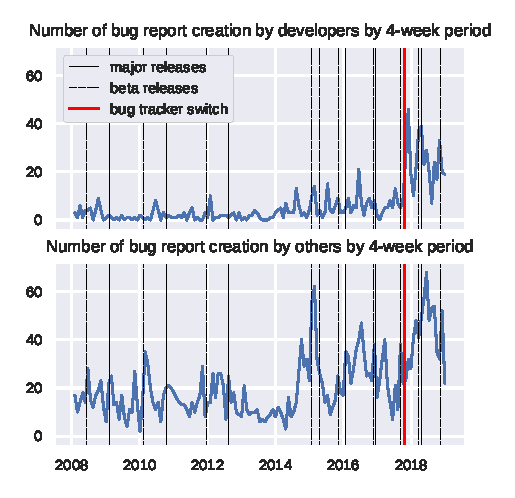
\includegraphics{bug_nb_with_releases.eps}
\caption{Number of issues per day (averaged by 4-week periods) with release dates (since 2016).} \label{bug_nb_with_releases}
\end{figure}

\begin{figure}
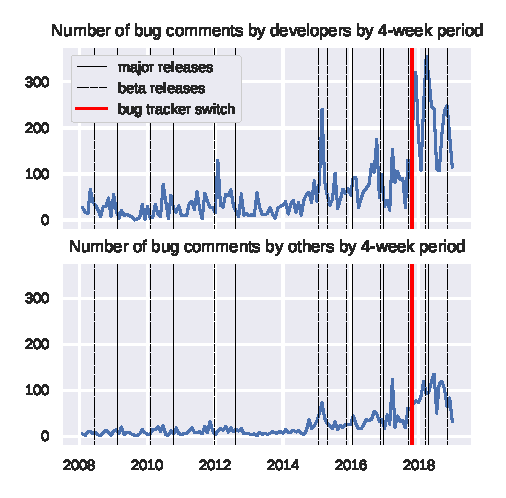
\includegraphics{comments_with_releases.eps}
\caption{Number of comments per day (averaged by 4-week periods) with release dates (since 2016).} \label{comments_with_releases}
\end{figure}

\begin{figure}
\includegraphics{reporters_with_releases.eps}
\caption{Number of weekly distinct reporters (averaged by 4-week periods) with release dates (since 2016).} \label{reporters_with_releases}
\end{figure}

\begin{figure}
\includegraphics{commentators_with_releases.eps}
\caption{Number of weekly distinct commentators (averaged by 4-week periods) with release dates (since 2016).} \label{commentators_with_releases}
\end{figure}

Considering the whole period (2016-2019), less issues are reported by developers than by non-developers. In a four-day period, on average, two issues are opened by developers and five by non-developers. On the other hand, developers post more comments than non-developers. On an average day, developers post around five comments and non-developers two. This is not surprising because some bugs found by developers are resolved directly without opening an issue and because issue reports are generally answered by developers.
There are more distinct non-developers than developers who open issues in an average week (around six distinct non-developers and two distinct developers).
On average on the whole period, there are slightly more distinct non-developers (per week) that comment than developers. Interestingly, this is a case where the switch of bug tracker has changed the ranking: before the switch there were more distinct developers that commented each week, and afterwards, there were more distinct non-developers.

For all outcomes, the mean before the switch is statistically significantly lower than the mean after the switch both for developers and non-developers (mean difference T-tests, $p < 0.001$). For some outcomes, the difference in activity patterns before and after the switch is clear to the naked eye. In Fig.~\ref{bug_nb_with_releases}, we see an increase in the number of issues reported by developers. In Fig.~\ref{comments_with_releases}, we see an increase in the number of comments by developers with many data points after the switch that are well above the highest point before the switch. Finally, in Fig.~\ref{commentators_with_releases}, we see a clear increase in the number of distinct non-developer commentators with almost all points after the switch above almost all points before the switch. Some other differences may be appreciated but are less clear to the naked eye than those presented.

\section{Methodology}
\label{methodology}

\subsection{Quantitative}
We exploit the fact that the switch from Bugzilla to GitHub can be seen as a clear cutoff in time to use a temporal sharp regression discontinuity design (RDD) to estimate the effects of the switch on our outcome variables; to determine if the estimated effects are statistically significant; and to interpret them causally.
The idea behind the RDD is that factors that influence bug tracking activity are fairly similar just before and just after the cutoff, which makes the differences observed between just before and just after the cutoff a consequence of the change that occurred at the cutoff (i.e., the switch of bug tracker).

The assumption behind this analysis is that reporters did not choose the exact moment in which the switch would take place. In the absence of any other discontinuity, the changes in the behavior of reporters just before and just after the migration is likely to depend mainly on the switch: the other factors influencing bug tracking activity evolve slowly, and should be pretty similar just before and just after the switch. It is important to note that estimated effects using this method will inform of the effect near the threshold (i.e., it will only give the Local Average Treatment Effect --LATE-- of the switch). Indeed, in the same way that behavior just before and just after the threshold is not likely to be different in the absence of the switch, the behavior several periods before and several periods after is likely to be different even in the absence of the switch. See~\cite{angrist2014mastering,angrist2008mostly} for an accessible and intuitive introduction to RDD; and~\cite{lee2010regression,jacob2012practical} for further details and a practitioner's guide to its empirical application.

We model the evolution of the bug tracking activity around the switch by two different functions, one before and one after the switch, fitted using Ordinary Least Squares~\cite{wooldridge2015introductory}. Their purpose is to accurately estimate the value at the switch in the absence and presence of treatment. Since only their value around the cutoff is relevant, we can choose to estimate them on a restricted bandwidth (number of periods) around the cutoff, or on a larger dataset. We also have the choice of different functional forms for these models.

In the context of an RDD, the choice of the bandwidth of the analysis and the functional form of the regression is always difficult. On the one hand, including data points that are far from the cutoff (in our case the bug tracker switch) will increase precision as it will reduce standard errors (because we will have more data points). On the other hand, including those points can bias estimation near the cutoff if the functional form of the evolution in the absence of switch is not accurately specified. Our main specification takes a conservative approach with a relatively small bandwidth of 175 days before and after the switch to minimize possible bias, and a simple linear model to avoid overfitting. However, as a robustness check, we also estimate a quadratic model on a larger time frame (511 days on each side). This conservative approach reduces the statistical power of our analysis, increasing the probability of observing false negatives (being unable to detect an effect where such an effect exists).

We use time as rating variable\footnote{The rating variable, also called the running variable or the forcing variable, is the variable on which we observe the cutoff.} and we estimate the following regression:  
\begin{equation*}
\arraycolsep=0pt
\begin{array}{l}
\mbox{\emph{Number of issues}}_t = \\
\quad\quad \gamma_0 +\gamma_1 \times \mbox{\emph{Relative date}}_t
+ \gamma_2 \times \mbox{\emph{After switch}}_t \\
\quad\quad +~\gamma_3 \times \mbox{\emph{Relative date}}_t \times \mbox{\emph{After switch}}_t
+ \epsilon_t
\end{array}
\end{equation*}
\noindent where $\mbox{\emph{Number of issues}}_t$ is the total number of issues opened during the day $t$; $\mbox{\emph{Relative date}}_t$ is the number of days from the date of the switch (zero is the first period after the switch); $\mbox{\emph{After switch}}_t$ is a binary variable equal to one if $t$ is a period after the switch and zero otherwise; $\mbox{\emph{Relative date}}_t \times \mbox{\emph{After switch}}_t$ is called the interaction term and $\epsilon_t$ is the residual error. This is equivalent to estimating the following two regressions, respectively before and after the switch:
\begin{equation*}
\begin{array}{l}
\mbox{\emph{Number of issues}}_{t < 0} =\\
\quad\quad \gamma_0 + \gamma_1 \times \mbox{\emph{Relative date}}_t + \epsilon_p \medskip\\
\mbox{\emph{Number of issues}}_{t \geq 0} = \\
\quad\quad (\gamma_0 + \gamma_2) + (\gamma_1 + \gamma_3) \times \mbox{\emph{Relative date}}_t + \epsilon_t
\end{array}
\end{equation*}
We estimate this regression by Ordinary Least Squares~\cite{wooldridge2015introductory} and compute heteroscedasticity robust standard errors.\footnote{The errors $\epsilon_t$ are said to be heteroscedastic if their variances differ. The standard calculations for estimation errors assume equal variances~\cite{wooldridge2015introductory}.
} Coefficient $\gamma_0$ is the estimated value just before the cutoff and $\gamma_1$ the slope before the cutoff. Coefficients $\gamma_2$ and $\gamma_3$ are the estimates of interest and will tell us the jump of the number of issues just after the switch and the change in slope due to the switch respectively. 

We estimate this regression for two different sub-samples: the developers and the non-developers. We replicate this analysis for all our outcome variables by changing the variable on the left hand side of the equation. 

\subsection{Qualitative}

In order to obtain qualitative insights into the effects of the switch that will help us interpret the quantitative results, we conducted semi-structured interviews of all developers of Coq that were active at the time of the switch (as defined in section \ref{data}) and that we included in our quantitative analysis. A total of 9 interviews were conducted between Mar., 19\textsuperscript{th} and Apr., 4\textsuperscript{th} 2019.
The two co-authors were present during the interviews and all the interviews were recorded. The answers were coded by both authors in an attempt to minimize errors. The interview outline with questions asked to all developers, and the encoding of the answers can be found in the supplementary material. 

\section{Quantitative results}
\label{results}
\subsection{Impact on the number of issues}

\begin{table}
\centering
\caption{Estimated impact on the number of issues. Statistically significant results are in boldface (\textbf{*} means $p<0.05$, \textbf{**} means $p<0.01$, \textbf{***} means $p<0.001$). Standard error is in parentheses.}
\label{tab:bug_nb}
\begin{tabular}{|r|c|c|c|}
\hline
&  Total & Developers & Non-developers \\
\hline
$\mbox{\emph{After switch}}_p$ & 0.629 & \textbf{0.73**} & -0.101 \\
 & (0.354) & (0.239) & (0.244) \\
\hline
$\mbox{\emph{Relative date}}_p$ & 0.00114 & -0.000383 & 0.00152 \\
$\times \mbox{\emph{After switch}}_p$ & (0.00341) & (0.00227) & (0.00245) \\
\hline
$\mbox{\emph{Relative date}}_p$ & 0.00305 & -0.00013 & \textbf{0.00318*} \\
 & (0.00182) & (0.000816) & (0.00157) \\
\hline
Constant & \textbf{1.23***} & \textbf{0.269***} & \textbf{0.96***} \\
 & (0.21) & (0.0809) & (0.181) \\
\hline
Observation number & 350 & 350 & 350 \\
\hline
\end{tabular}
\end{table}

\begin{figure}
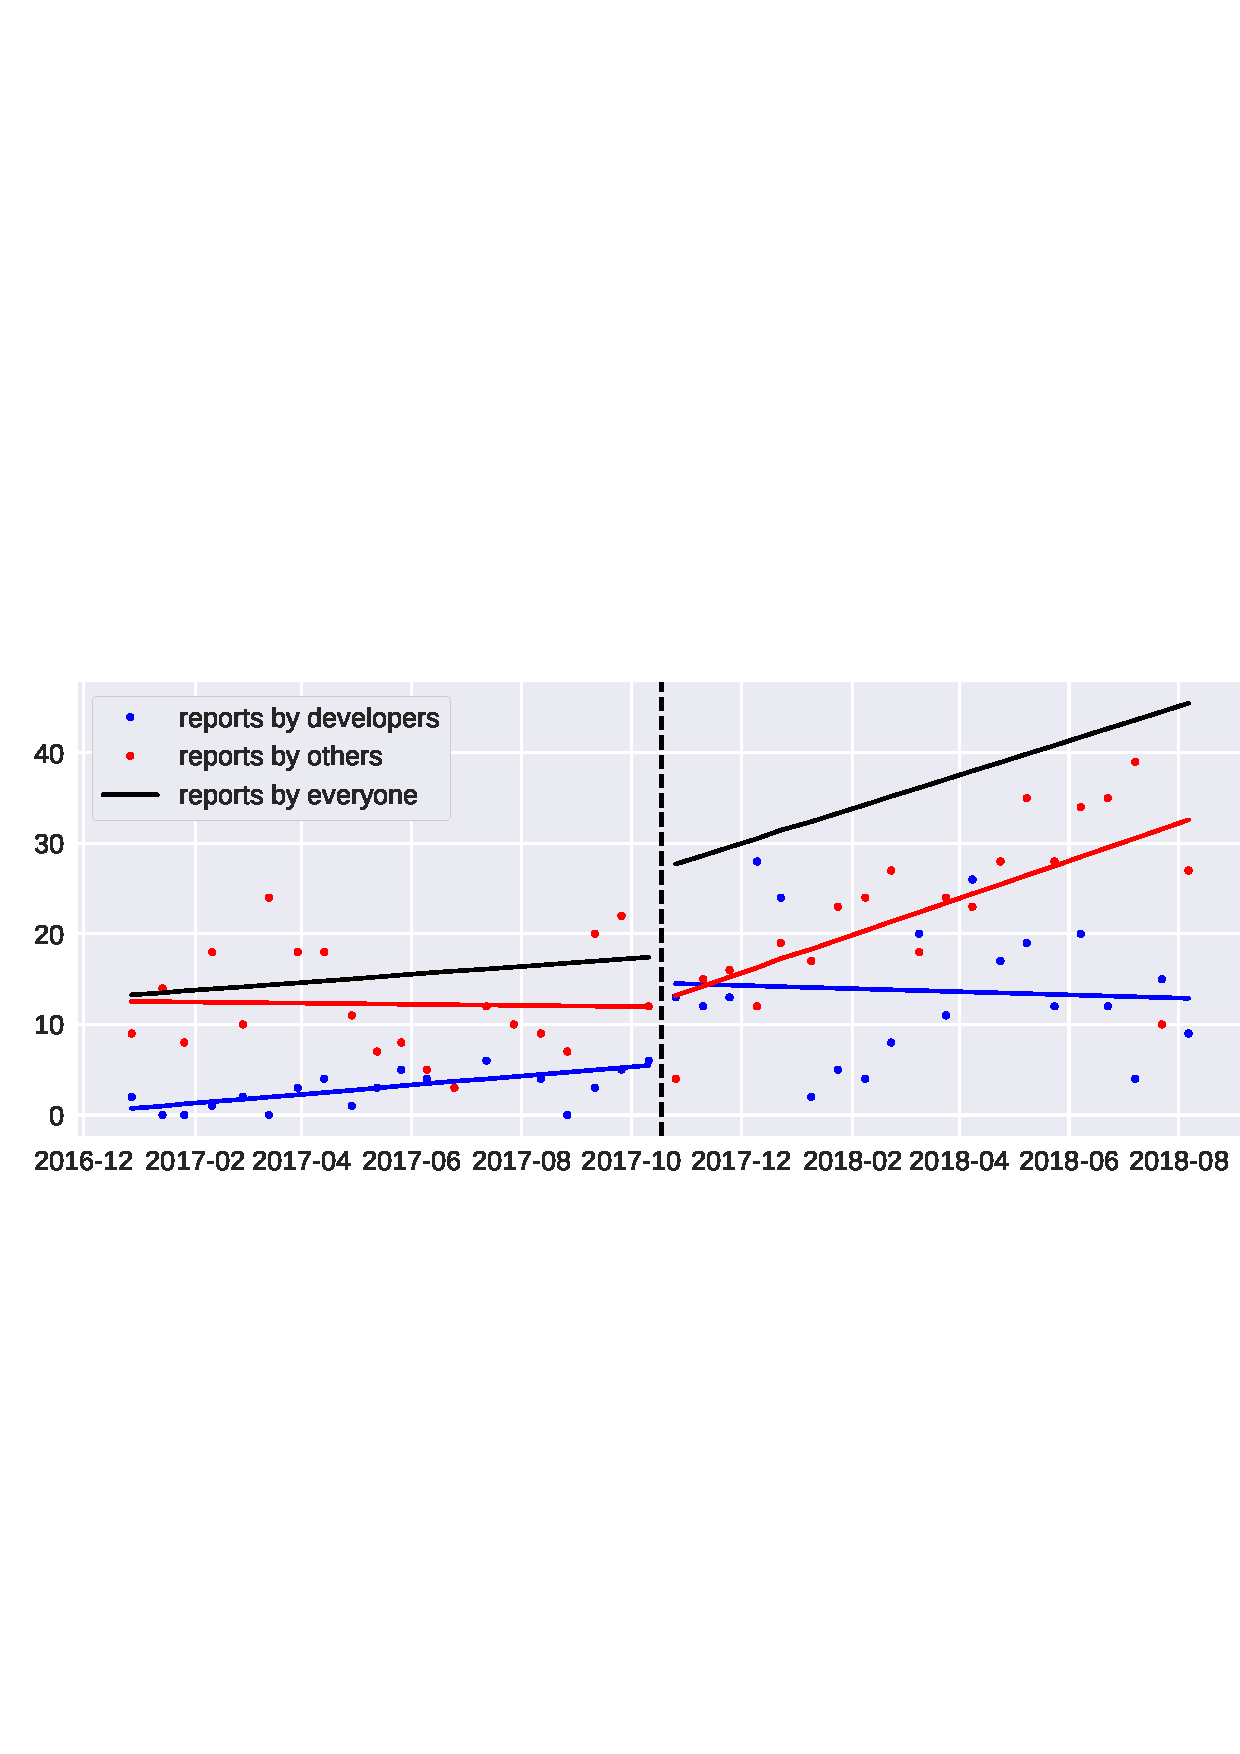
\includegraphics{bug_nb_rd.png}
\caption{Number of issues per day before and after the switch (with fitting lines and confidence intervals from the regression results, and points corresponding to average values over two-week periods).} \label{bug_nb_rd}
\end{figure}

Table~\ref{tab:bug_nb} presents the estimated impact of the switch on the number of issues. Each column shows the estimates for a different sub-sample (all reporters, developers and non-developers). Asterisks represent levels of statistic significance. We interpret results as significant if the p-value is below 0.05. Estimates that are not statistically significant cannot be interpreted as an absence of effect but indicate that if such effect exists, we are unable to discern it with our conservative approach. Fig.~\ref{bug_nb_rd}  shows the number of issues before and after the switch and the fitting lines and confidence intervals corresponding to the regression results. 

For developers, we see a statistically significant positive jump in issues just after the switch. The switch is estimated to have increased the daily number of issues by 0.7 (representing an increase of around 270\%). That is, on average, we observe around one issue opened by developers every day after the switch,
while, before the switch, developers opened an issue every four days. There is no statistically significant effect on the number of issues by non-developers.

\subsection{Impact on the number of comments}

Table~\ref{tab:comment_nb} and Fig.~\ref{comment_nb_rd} show the estimated impact of the bug tracker switch on the number of comments. We see a statistically significant positive jump. The number of comments just after the switch more than doubles (from around 5 comments per day before the switch to around 10 after). This appears to be, for the most part, due to comments by developers who increased their average number of comments per day from around 3 to around 8.

\begin{table}
\centering
\caption{Estimated impact on the number of comments. Statistically significant results are in boldface (\textbf{*} means $p<0.05$, \textbf{**} means $p<0.01$, \textbf{***} means $p<0.001$). Standard error is in parentheses.}
\label{tab:comment_nb}
\begin{tabular}{|r|c|c|c|}
\hline
&  Total & Developers & Others \\
\hline
$\mbox{\emph{After switch}}_p$ & 5.5* & 4.76** & 0.739 \\
 & (2.24) & (1.79) & (0.717) \\
\hline
$\mbox{\emph{Relative date}}_p$ & 0.0155 & 0.0144 & 0.00112 \\
$\times \mbox{\emph{After switch}}_p$ & (0.0205) & (0.017) & (0.0063) \\
\hline
$\mbox{\emph{Relative date}}_p$ & 0.00147 & -0.00288 & 0.00435 \\
 & (0.00882) & (0.00673) & (0.00383) \\
\hline
Constant & 4.77*** & 2.95*** & 1.82*** \\
 & (1.03) & (0.704) & (0.463) \\
\hline
Observation number & 360 & 360 & 360 \\
\hline
\end{tabular}
\end{table}

\begin{figure}
\includegraphics{comment_nb_rd.png}
\caption{Number of comments per day before and after the switch (with fitting lines and confidence intervals from the regression results, and points corresponding to average values over two-week periods).} \label{comment_nb_rd}
\end{figure}

\subsection{Impact on the number of distinct reporters}

Table~\ref{tab:reporters} and Fig.~\ref{reporter_nb_rd} show the estimated impact of the switch on the number of distinct issue reporters each week. These results show that the switch had also a positive effect on the number of distinct developer-reporters in a given week. The number of distinct developers that opened an issue in a given week increased, on average, by around 130\% (from 1.5 developer-reporters each week before the switch to 3.42 after).

\begin{table}
\centering
\caption{Estimated impact on the number of weekly distinct reporters. Statistically significant results are in boldface (\textbf{*} means $p<0.05$, \textbf{**} means $p<0.01$, \textbf{***} means $p<0.001$). Standard error is in parentheses.}
\label{tab:reporters}
\begin{tabular}{|r|c|c|c|}
\hline
&  Total & Developers & Non-developers \\
\hline
$\mbox{\emph{After switch}}_p$ & 2.17 & \textbf{1.92*} & 0.245 \\
 & (1.68) & (0.977) & (1.27) \\
\hline
$\mbox{\emph{Relative date}}_p$ & 0.146 & 0.0162 & 0.13 \\
$\times \mbox{\emph{After switch}}_p$ & (0.108) & (0.0648) & (0.0862) \\
\hline
$\mbox{\emph{Relative date}}_p$ & 0.0608 & -0.00462 & 0.0654 \\
 & (0.0903) & (0.0378) & (0.0675) \\
\hline
Constant & \textbf{6.03***} & \textbf{1.5**} & \textbf{4.53***} \\
 & (1.47) & (0.579) & (1.11) \\
\hline
Observation number & 50 & 50 & 50 \\
\hline
\end{tabular}
\end{table}

\begin{figure}
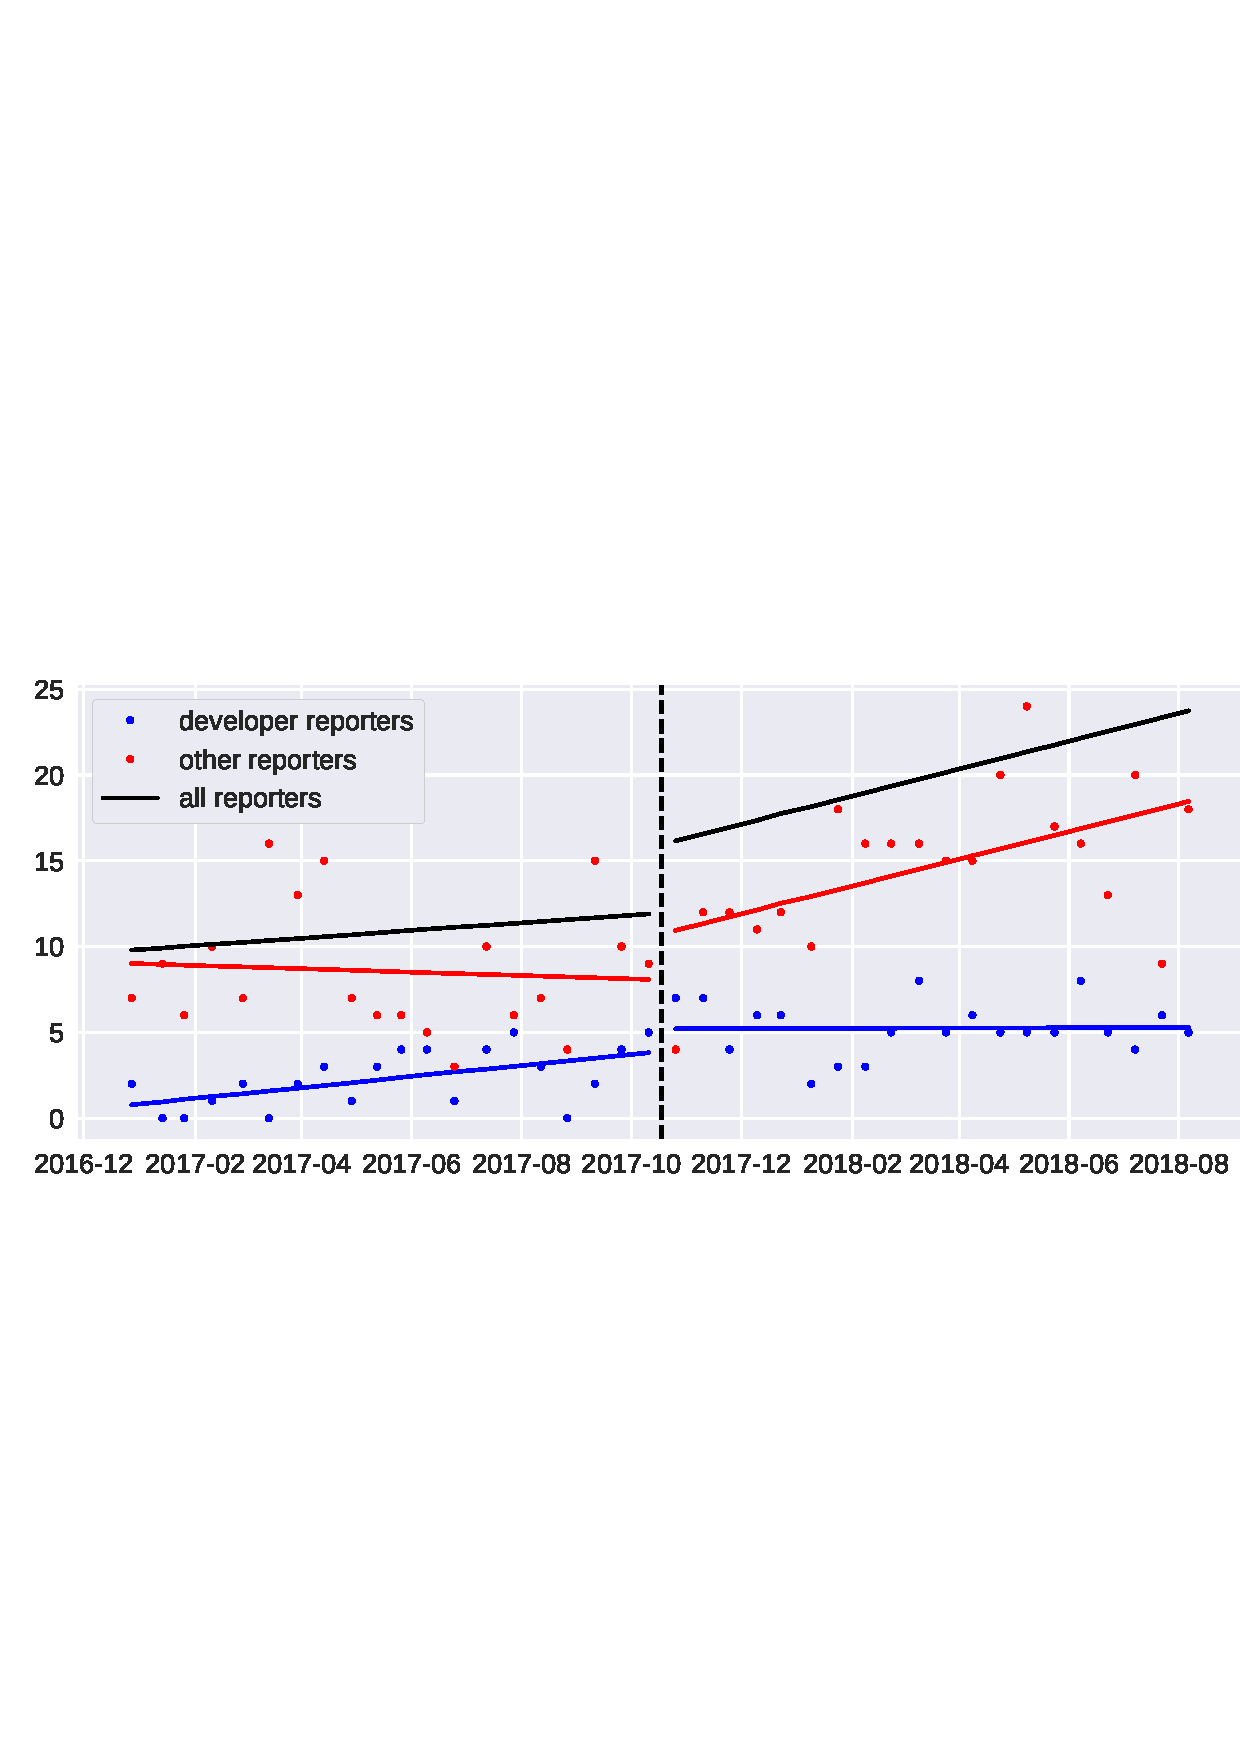
\includegraphics{reporter_nb_rd.png}
\caption{Number of weekly distinct reporters before and after the switch (with fitting lines and confidence intervals from the regression results, and points corresponding to average values over two-week periods).} \label{reporter_nb_rd}
\end{figure}

\subsection{Impact on the number of distinct commentators}

Table~\ref{tab:commentators} and Fig.~\ref{commentator_nb_rd} show the estimated impact of the switch on the number of distinct commentators each week. We observe a statistically significant jump in the number of both developer and non-developer commentators. 

In general terms, the number of distinct commentators in a given week changed from an average of 7 to an average of 13 (almost doubling the commentators). This increase is due in larger part to the number of non-developers commentators, which more than doubles (from around 3 to around 7 on an average week), while, among developers, the number of commentators  increases by 66\% (from around 4 to around 6).

\begin{table}
\centering
\caption{Estimated impact on the number of weekly distinct commentators. Statistically significant results are in boldface (\textbf{*} means $p<0.05$, \textbf{**} means $p<0.01$, \textbf{***} means $p<0.001$). Standard error is in parentheses.}
\label{tab:commentators}
\begin{tabular}{|r|c|c|c|}
\hline
&  Total & Developers & Non-developers \\
\hline
$\mbox{\emph{After switch}}_p$ & 6.19*** & 2.53* & 3.66** \\
 & (1.81) & (1.05) & (1.17) \\
\hline
$\mbox{\emph{Relative date}}_p$ & 0.205$\dagger$ & 0.0769 & 0.128 \\
$\times \mbox{\emph{After switch}}_p$ & (0.118) & (0.0641) & (0.0924) \\
\hline
$\mbox{\emph{Relative date}}_p$ & -0.0692 & -0.0469 & -0.0223 \\
 & (0.0833) & (0.0589) & (0.0463) \\
\hline
Constant & 7.06*** & 3.83*** & 3.23*** \\
 & (1.54) & (0.984) & (0.861) \\
\hline
Observation number & 50 & 50 & 50 \\
\hline
\end{tabular}
\end{table}


\begin{figure}
\includegraphics{commentator_nb_rd.png}
\caption{Number of weekly distinct commentators before and after the switch (with fitting lines and confidence intervals from the regression results, and points corresponding to average values over two-week periods).} \label{commentator_nb_rd}
\end{figure}

\subsection{Impact on the number of new reporters and commentators}

We refer the reader to the companion Jupyter notebook for the results on new reporters and new commentators. The estimated coefficients also show a positive jump, but they are not statistically significant.

\section{Research questions discussion}
\label{discussion}

\subsection{RQ1: Impact on level of bug tracking activity}

In Sec.~\ref{descriptive-stats}, we observed an increase in the mean number of issues and comments after the switch, both for developers and non-developers. However, as shown in Sec.~\ref{results}, we are able to find a causal effect of the switch on these two variables only for developers. In particular, the estimated impact of the switch was to more than quadruple the number of opened issues, and to more than double the number of comments, by developers. This significant increase in the bug tracking activity is all the more remarkable given that two (out of nine) developers highlighted that it was hard to adapt to the new bug tracker, and thus they reduced their activity after the switch.

We not only observed an increase in activity by developers but also an increase in the number of distinct developer reporters and commentators. This shows that developers are active more often.

When we asked developers how they would interpret this effect on the level of activity of developers, they almost all (7 out of 9) mentioned the more comfortable experience of using GitHub's integrated bug tracking system, reminding many of the motivations they had previously listed for switching (better interface, less slow, no switching between issues and pull requests, etc.). Many developers told us that they personally did not always opened issues on the Bugzilla bug tracker when they found small bugs, and they now did open issues more often because it was easier to do so. One developer in particular admitted he had not been very active on the Bugzilla bug tracker since the main development activity had moved to GitHub's pull requests.

In addition, the GitHub notification system (including the mention system which allows attracting a developer's attention on a specific issue) was identified as being responsible for part of the additional activity. When a user is subscribed to a repository (which is the case of most Coq developers), notifications (by e-mail or in the web interface) are sent whenever a new issue is opened or a comment is posted. This can attract the attention of developers more quickly and lead to more comments in response. It was mentioned how some developers had trouble adjusting their settings to make it easier to manage this large flow of information (GitHub's notification default settings are quite unsuited to repositories with large levels of activity).

\subsection{RQ2: Impact on quality of bug tracking activity}

Measuring quality of bug tracking activity is difficult. That is why we could only answer this second research question qualitatively, by asking developers if their perceived a change in quality of issue reports and interactions on the bug tracker. A majority (5 out of 9) claimed that GitHub helped at least some reporters produce better issue reports (thanks in particular to formatting and the issue template\footnote{GitHub allows setting up a template to help users opening issues know what information they should provide~\cite{github_issue_template}.}). However, three developers added that the switch had also attracted less experienced users whose reports were sometimes of a lower quality.

Regarding the quality of interactions on the bug tracker, again a majority of developers (6 out of 9) claimed that it improved after the switch. In particular, it was mentioned that users are more reactive and answer more frequently when they are asked additional information.
Several developers also emphasized that it was easier to discuss on the new platform, especially with respect to bugs that cross project boundaries. Indeed, GitHub makes it easy to link between issues, not only in the same repository, but also across the repositories of multiple projects. Examples of related projects include projects that Coq depends on (the OCaml compiler, the camlp5 pre-processing library, the Sphinx documentation tool, etc.) and projects that depend on Coq (a variety of Coq plugins and libraries, editor support packages, etc.).

Other perceived quality improvements include an easier navigation among issues, which helps both developers do a more efficient triaging, and users discover existing issues more easily, on which they can subsequently leave comments adding information. This participation of users is useful to improve the overall quality of some preexisting reports.

\subsection{RQ3: Impact on the audience of the bug tracker}

In Sec.~\ref{descriptive-stats}, the clearest change after the bug tracker switch was the increase in the number of distinct weekly non-developer commentators. This observation was further confirmed in Sec.~\ref{results}: the estimated impact of the switch was to more than double the number of distinct non-developer commentators in an average week.

When asked to interpret
this surge,
all the developers said that GitHub was more accessible, either because it is a very popular platform on which many people already have an account (especially computer science students who represent a large number of Coq users), or because it is quite simple to use, especially in comparison with Bugzilla. These explanations apply to a general increased participation of non-developers, but do not explain specifically an increase in the number of distinct commentators (as opposed to reporters).

Some factors that were mentioned by a few developers and could have specifically influenced the number of commentators are that some external contributors who already contributed through pull requests now also comment issues more systematically, that more attention is given to newcomers, that there is generally more discussion between developers and non-developers on the bug tracker, and that it is easier for interested users to subscribe to just part of the bug tracking activity (and thus participate to the discussion without following the activity on the whole bug tracker).

\subsection{General discussion}

Beyond the scope of our research questions, we gathered other perceived effects of the bug tracking switch that affect the quality of software development in a broader way. Most of the developers we interviewed noted that the bug tracker switch to GitHub contributed to a more general culture switch towards a more recorded communication and transparent development. In particular, it was mentioned that GitHub makes written communication less costly, that the mention system can be used in place of personal e-mails, which avoids losing technical content in private threads, and that more types of discussion take place in the bug tracker (included related to long-term plans or development processes).

In addition, some developers found that GitHub provides a more global view of the state and history of development. They also perceived an increased visibility of developers' own work, and of the Coq project overall.  

While our RDD methodology can only be used to measure the immediate causal impact, an important question concerns the long-term effect of the switch. Our descriptive statistics (Sec.~\ref{descriptive-stats}) and robustness checks on longer time horizons (Sec.~\ref{threats}) seem to validate that the observed effect of the switch was durable. This can be explained in part because GitHub evolves faster, according to the needs of ever-evolving open source developing processes. During our interviews, we learned that some of the recently added features of GitHub are particularly appreciated.

\section{Robustness checks and threats to validity}
\label{threats}
\subsection{Internal validity and robustness checks}

The most important threat when performing RDDs, especially on time-series, is to have another event that occurred near the cutoff, and which could have influenced the outcomes. In our case, there were no such events that we could identify, except the 8.7.0 release, that took place on Oct. 17\textsuperscript{th}, just one day before the switch.
To confirm that it is not the release that is driving our results, we perform some placebo robustness checks, i.e. we do the exact same analysis that we do for the bug tracker switch, replacing the cutoff date by the date of six other releases (all the other major releases since 2009, except the latest one because we do not have yet enough data points after the release). We show that the only positive and significant effect in the bug tracker activity after any proposed cutoff is the effect after the switch. For some outcomes, we observe a significant effect after some major releases but this effect is negative and of a much lower absolute magnitude. It is thus very unlikely that our results are driven by the release close to the switch and not by the switch itself.  

Our main specification for RDD uses a small bandwidth and a linear model. As a robustness check, we estimate our model using larger time horizons (511 days, i.e. 73 weeks, on each side of the cutoff, corresponding to all the data that we collected after the switch and the same number of days before). To reduce the associated bias, we include a quadratic term to allow the regression to better fit the data and ``adjust'' to far away data points. Following Gelman et al. ~\cite{gelman2018high}, we include only a quadratic polynomial and not a polynomial of a higher order. Virtually all our results still hold with this specification, with comparable estimated magnitude, and with statistical significance (with only the number of distinct developer-reporters going just above the arbitrary $0.05$ p-value threshold).

Temporal RDDs have some notable differences from other types of RDDs, as noted in a recent paper by Hausman and Rapson \cite{hausman2018regression}. One major difference is the capacity of anticipation and adaptation to the treatment, that affects directly the outcome. To ensure that our results are robust to these effects, we additionally estimate donut RDDs (i.e. we exclude the data points just after and just before the switch, which are potentially problematic), as recommended in \cite{hausman2018regression}. Our results still hold with comparable estimated magnitudes, and a few of them going just above the arbitrary $0.05$ p-value threshold (this is not unexpected, given that we have removed data points, and this automatically increases the standard errors).
Time-series are also subject to potential serial auto-correlation of errors (errors at time $t+1$ are not independent from errors at time $t$). Failing to take such auto-correlation into account can lead to underestimate standard errors. To check that there is no serial auto-correlation in our data, we plot residuals\footnote{Residuals are the differences between measured and estimated values.}~\cite{wagner2002segmented}, and notice the absence of any specific pattern beyond those which show the presence of heteroscedasticity, which we already control for (see Jupyter notebook).

\subsection{External validity}

This is only a case study on a very specific project with a relatively small core team, and therefore it is very important that this study be replicated before we can draw general conclusions that can serve to formulate recommendations for open source developers. Our reusable assets, such as the migration tool and the analysis pipeline should be helpful to perform such replications.

\section{Conclusion and perspectives}
\label{conclusion}
We have conducted the migration of the Coq bug tracker from Bugzilla to GitHub and we have improved existing tooling in the process. Other open source projects have already benefited from this enhanced tooling (Ledger, migrating from Bugzilla to GitHub in 2018), or the experience that we drew from it (OCaml, migrating from Mantis to GitHub in 2019).

By analyzing mined repository data, we have shown that this bug tracker switch resulted in an increase in bug tracking activity in two ways. First, the developers are using the bug tracker more, by opening more issues and communicating more. Second, the non-developers are more numerous to take an active role by commenting issues as well.

We complemented this quantitative analysis by interviewing the developers. Almost all of them were very happy with the bug tracker switch. They provided us with insights to explain our estimated causal effects in bug tracking activity, and on the more general impact on the development process and its transparency.

Finally, we presented and explained an example of the use of RDD, an econometric method to derive causality, that is seldom used in empirical software engineering. We believe that there are many cases where this methodology would be useful to help demonstrate causality from mined software repository data.

Given the lack of literature on the effects of bug tracking environments, interested researchers could expand our analysis in many different ways. Analyzing other outcomes (such as pull requests or the rapidity of bug resolution) could give interesting additional insights, and help create a more complete picture of the mechanisms at play.
Replicating our analysis on more projects would increase the external validity of the results, and allow researchers to offer clear takeaways to projects interested in switching their bug trackers. Based on this first study, it seems that moving to a more popular, and integrated platform can help increase the level, the quality and the audience of bug tracking activity. \\

\scriptsize
\noindent \footnotesize{\textbf{Supporting data.}}
Supplementary materials can be found at \url{https://github.com/Zimmi48/impact-of-switching-bug-trackers/tree/icsme-final}. They include our extraction and analysis code in a Jupyter notebook, the bug tracking data gathered from GitHub, the interview questions and coding of the answers.

\noindent\footnotesize{\textbf{Acknowledgements.}}
We would like to thank Ambre Williams for valuable advice and help on the design and implementation of the data analyses, C\'ecile Rottner for general advice, support, and proof-reading, and Yann R\'egis-Gianas for encouragements and guidance.
We would also like to thank the anonymous reviewers from MSR 2019 and ICSME 2019 for valuable feedback.
Finally, we would like to thank Andriy Berestovskyy for providing the Bugzilla import tool, and Martin Michlmayr for performing the first steps in porting our modifications upstream.
%
% ---- Bibliography ----
\balance
\bibliography{bib}
\bibliographystyle{IEEEtran}
%
\end{document}
